\chapter{Design and Implementation}
\label{chap:design}
\section{Docker}
In native Docker, It has two part, Docker Client and Docker Daemon. Docker Daemon has many components include server, engine, registry, graph, driver and runC. To  support dump checkpoint and restore request, some of these steps should be implemented.

\subsection{Docker Client}
We implement 3 Docker commands in Docker Client, including checkpoint, restore, migrate. In checkpoint command should have these configurations:
\begin{itemize}
	\item image directory - Dump checkpoint image directory.
	\item work directory - Dump checkpoint image log directory.
	\item leave running - After dumping checkpoint image, keeping running container or not.
	\item pre-dump - Pre-dump checkpoint memory image to minimize frozen time.
	\item pre image directory - Define which version image to compare.
	\item track memory - Track memory to pre image directory image to minimize disk space.
\end{itemize}
In restore command should have these configurations:
\begin{itemize}
	\item image directory - Checkpoint image directory to restore from.
	\item work directory - Directory for restore log.
	\item force - Fore restoring container from image directory whether container is running or not.
\end{itemize}
In migrate command, it focus on Docker Swarm Scheduler filter configurations. In run command, we can do this with the environment variable or the label. Therefore, we implement environment variable and the label configurations in migrate command.

\subsection{Docker Daemon}
In native Docker Daemon, it doesn't support checkpoint and restore command.
Fortunately, it is already implemented in runC, so we have to add some code to proxy Docker Client's requests through Docker Daemon to runC.

\section{Docker Swarm configuration}
As Figure \ref{fig:Docker Swarm with remote storage server}, we prepare a remote storage server for saving Docker containers dump checkpoint images. It should have fault tolerant to avoid service shout down. For these reasons, We choose glusterFS to be our experiments remote storage server.                            

After setting up glusterFS, we mount it to every Docker nodes in the same folder. To avoid mount it as absolute path in every Docker nodes, we mount it to Docker root which we can change configuration in Docker Daemon.

\begin{figure}[h]
\begin{center}
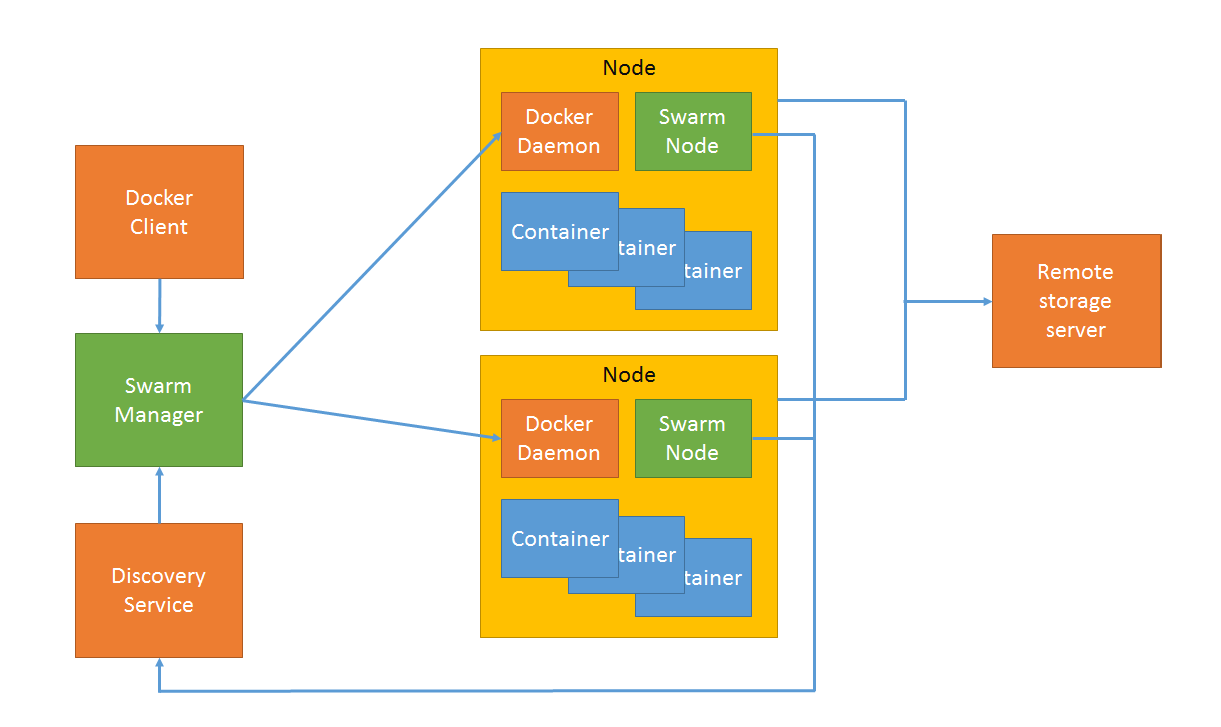
\includegraphics[width=15cm]{figure/swarm_docker_remote.png}
\end{center}
\caption{Docker Swarm with remote storage server}
\label{fig:Docker Swarm with remote storage server}
\end{figure}

\section{Docker containers migration in Docker Swarm}
Docker Swarm creates containers through Swarm scheduler to dispatch Docker nodes. If we want to specific assign which node we want to create containers, we have to set filters like constraint, affinity or dependency.
To migrate containers in Docker Swarm, we must avoid the containers which we want to migrate that migrate to an other nodes, instead of the same node.
\begin{enumerate}[Step 1.]
	\item Check Docker Swarm cluster has at least two Swarm nodes.
    \item Parse Docker Client requests to analyse label and environment variables, and transform label and environment variables to Docker Swarm filters.
    \item Add constraint filter to make sure the container which we want to migrate does not migrate to the same node.
    \item Pre-dump the container checkpoint image which we want to migrate to decrease container frozen time.
    \item Dump the container checkpoint image by tracking memory from pre-dump checkpoint image.
    \item Create empty container on the Docker Swarm scheduler chooses node.
    \item Restore the container to the Docker Swarm scheduler chooses node.
    \item Delete the checkpoint images.
    \item If the container was migrated which had setted checkpoint restore rescheduling policy, it will restart checkpoint restore rescheduling policy \ref{sec:checkpoint restore rescheduling policy}.
\end{enumerate}

\section{Docker Swarm checkpoint restore rescheduling policy}
\label{sec:checkpoint restore rescheduling policy}
In Docker Swarm, it has rescheduling policy. As we set the reschedule policy when we start a container, whenever Swarm nodes fail, Swarm Manager will restart the containers which on the fail nodes to another alive Swarm Nodes.

We improve this policy that we checkpoint every containers which we want to keep checkpoint for every checkpoint ticker. Whenever Swarm Nodes fail, Swarm Manager will restore the containers which Swarm manager has dumped checkpoint. Otherwise, restore rescheduling policy provides version checkpoint by memory track. It only dump different memory page checkpoint to new version checkpoint.

In addition, it also support high availability that whenever Docker Swarm primary manager fails, the others Swarm Manager replica instances will lead a new primary manager. After replica leading a new primary manager, it will restart container checkpoint tickers.
%By experment, it can save at least XX% hard disk space

\subsection{Docker Swarm container checkpoint tickers}
\begin{enumerate}[Step 1.]
	\item Set checkpoint-time label and keep version label when we create the container.
    \item Swarm Manager analyzes checkpoint label when the container has created. If keep version label isn't setted, keep version will be setted to 5.
    \item After the container starting, starting the container checkpoint ticker. Container checkpoint tickers are for when users want to checkpoint container repeatedly at regular intervals. Container checkpoint tickers will do these steps:
    \begin{enumerate}[Step a.]
    \item Swarm Manager sends pre-dump checkpoint request to Swarm Node's Docker Daemon when every Pre-dump version start.
    \item After pre-dumping the container, Swarm Manager sends dump new version checkpoint request to Swarm Node's Docker Daemon. Every new checkpoint images track memory to last checkpoint version image, just save memory difference in new checkpoint image. We save keep-version(default 5) versions in the same directory(Figure \ref{fig:Containers checkpoint versions in remote storage server}).
    \item Send delete checkpoint request to Swarm Node's Docker Daemon to delete last Pre-dump version directory whenever container has two Pre-dump versions.
    \end{enumerate}
\end{enumerate}
\begin{figure}[h]
\begin{center}
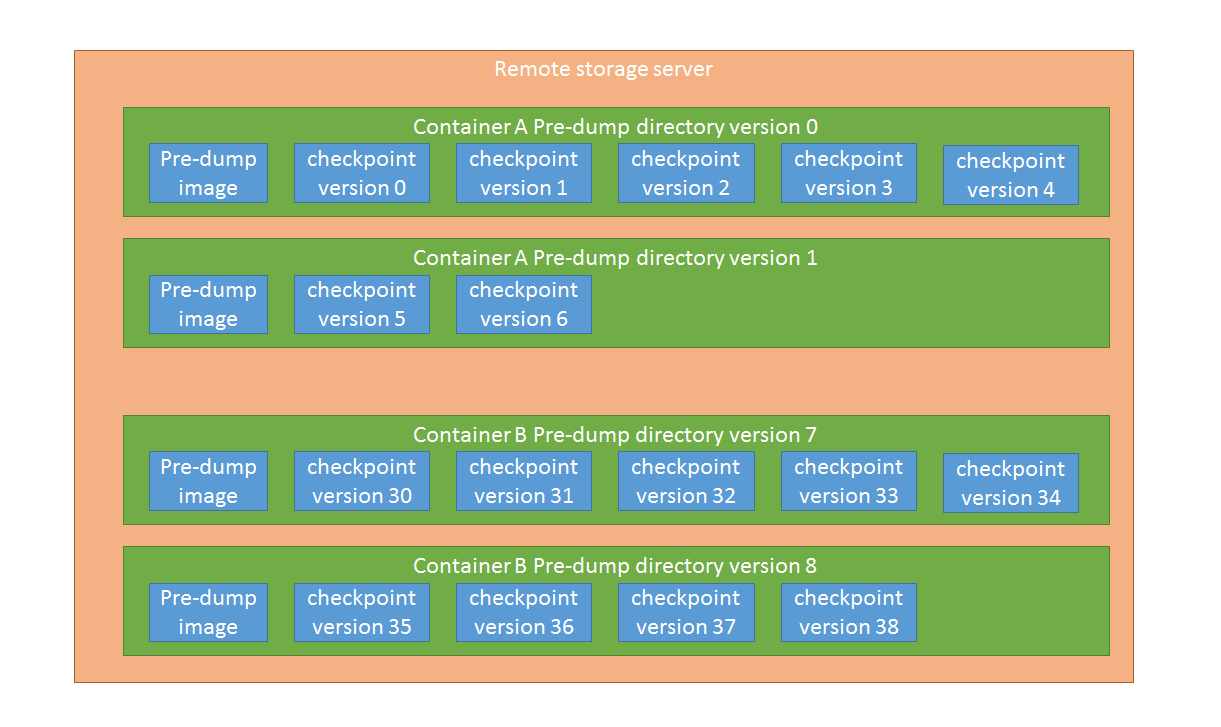
\includegraphics[width=15cm]{figure/checkpoint_demo.png}
\end{center}
\caption{Containers checkpoint version in remote storage server}
\label{fig:Containers checkpoint versions in remote storage server}
\end{figure}
\subsection{Docker Swarm restore rescheduling policy}
\begin{enumerate}[Step 1.]
	\item Set reschedule:restore label when we create the container.
	\item Swarm Manager analyzes restore label when the container start.
    \item Whenever Swarm Nodes fail, Swarm Manager will restore the containers which Swarm Manager has dumped checkpoint last version to another Swarm nodes.
    \item To avoid dumping checkpoint version failing at the same time, if restoring last version failing, Swarm Manager will retry second last version checkpoint to restore. It will retry keep-version(default 5) times.
    \item If Swarm Manager retries keep-version are all fail, it will create and start a new container as normal Docker Swarm rescheduling policy.
\end{enumerate}

\subsection{High availability of Swarm Manager in Docker Swarm checkpoint restore rescheduling policy}
Whenever Docker Swarm primary manager fails, the others Swarm Manager replica instances will lead a new primary manager. After replica leading a new primary manager, it searching every Docker Node's containers which has checkpoint restore rescheduling policy's label. If the containers has checkpoint restore rescheduling policy's label, Docker Swarm new primary manager will restart container checkpoint tickers.